\documentclass[a4paper]{article}

\usepackage{graphicx}
\usepackage{amsmath,amssymb}
\usepackage{minted}
\usepackage{multirow}
\usepackage{float}
\usepackage{todonotes}
\usepackage{forest}
\usepackage{xstring}
\usepackage{xcolor}
\usepackage[most]{tcolorbox}
\usepackage{xparse}
\usepackage{natbib}

\usetikzlibrary{graphs,graphdrawing}
\usegdlibrary{layered}

% for external graphviz
\input{/home/donkarlo/Dropbox/repo/nd_language_ai_project/src/nd_language_ai/formal/computer/programming/tex/latex/code_clips/external_graphviz.tex}

% for tags
\input{/home/donkarlo/Dropbox/repo/nd_language_ai_project/src/nd_language_ai/formal/computer/programming/tex/latex/part/control_sequence/kind/semtag/semtag.tex}

% for links
\input{/home/donkarlo/Dropbox/repo/nd_language_ai_project/src/nd_language_ai/formal/computer/programming/tex/latex/code_clips/seehere.tex}

\title{}
\date{}
\author{Mohammad Rahmani}

\begin{document}
   \maketitle
   \begin{figure}[H]
      \centering
      \includegraphics[width=0.9\textwidth]{s_11_u_5.png}
   \end{figure}

   \begin{figure}[H]
      \centering
      \includegraphics[width=0.9\textwidth]{s_11_u_5_mine.png}
   \end{figure}

   \section{Seit 12}
      \begin{figure}[H]
         \centering
         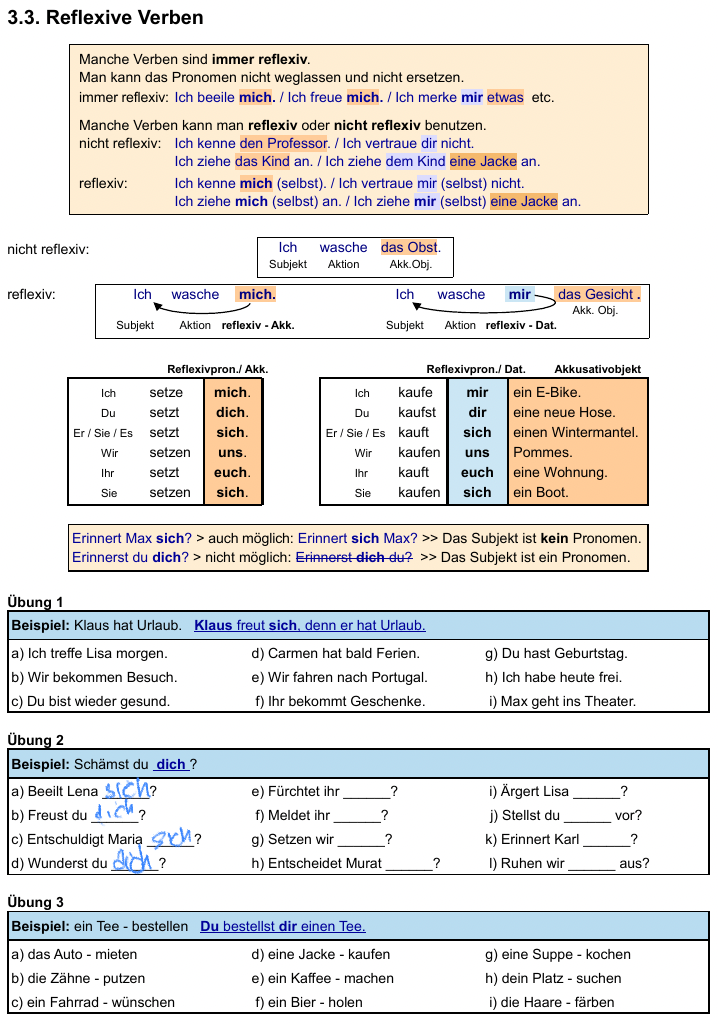
\includegraphics[width=0.9\textwidth]{img_1.png}
      \end{figure}

      reflexiv Verben
      \begin{figure}[H]
         \centering
         \includegraphics[width=0.9\textwidth]{img_0.png}
      \end{figure}
      \begin{figure}[H]
         \centering
         \includegraphics[width=0.9\textwidth]{s_12_u_1.png}
      \end{figure}
      \begin{figure}[H]
         \centering
         \includegraphics[width=0.9\textwidth]{img_2.png}
      \end{figure}

   \section{s_12_u_2}
      \begin{figure}[H]
         \centering
         \includegraphics[width=0.9\textwidth]{s_12_u_2.png}
      \end{figure}

   \section{s_12_u_3}
      \begin{figure}[H]
         \centering
         \includegraphics[width=0.9\textwidth]{s_12_u_3.png}
      \end{figure}
   \section{Lektion 4}
      \subsection{ Verben mit Präpositionalobjekt}
         \begin{figure}[H]
            \centering
            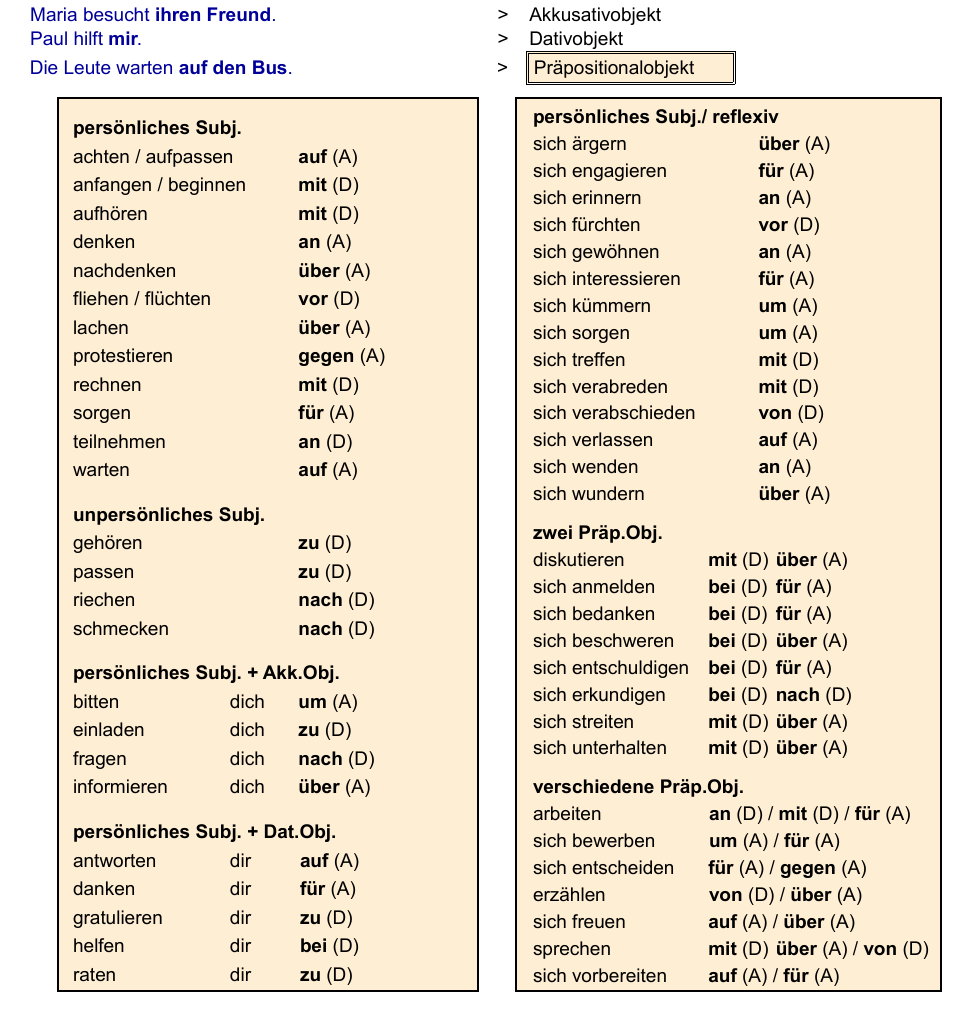
\includegraphics[width=0.9\textwidth]{img_3.png}
         \end{figure}
   \section{s_13_u_1}
      \begin{figure}[H]
         \centering
         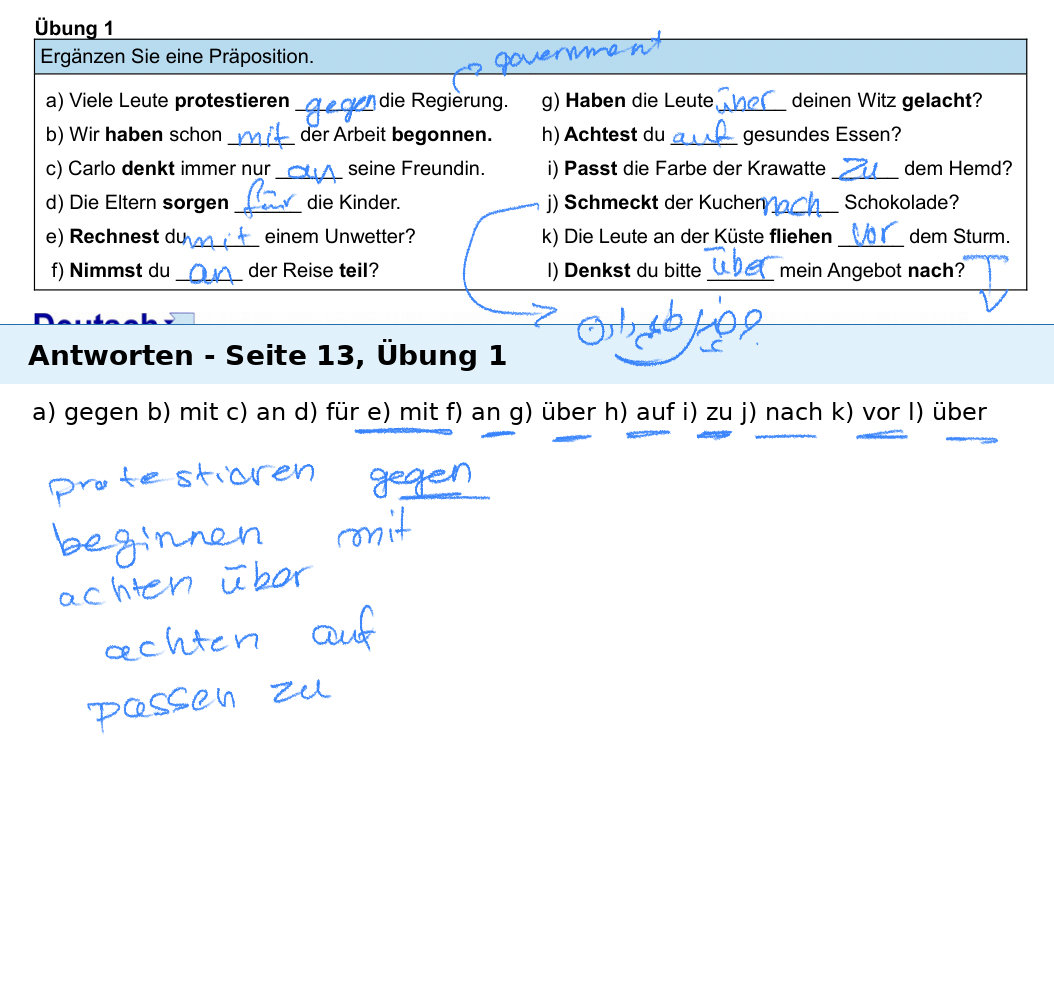
\includegraphics[width=0.9\textwidth]{s_13_u_1.png}
      \end{figure}
   \section{s_14_u_2}
      \begin{figure}[H]
         \centering
         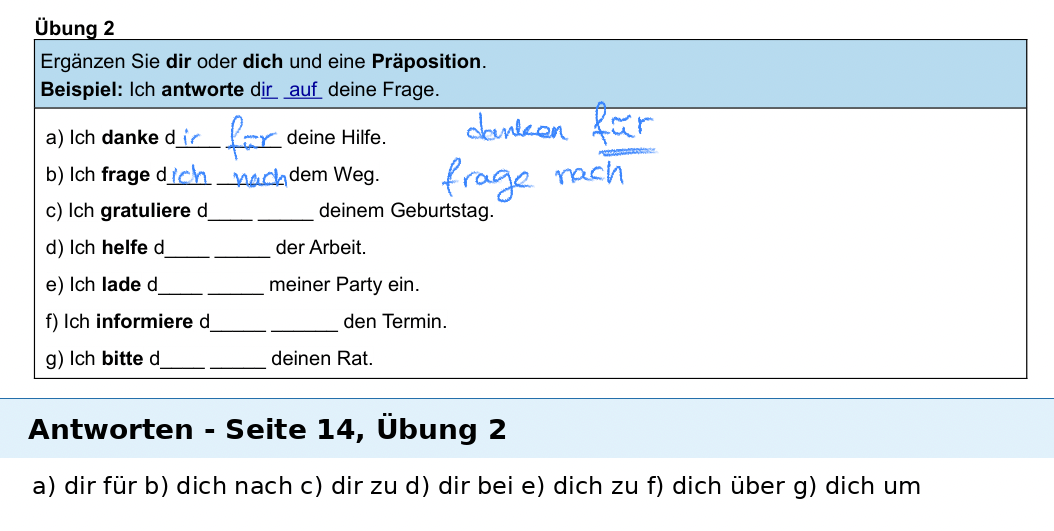
\includegraphics[width=0.9\textwidth]{s_14_u_2.png}
      \end{figure}
   \section{s_14_u_3}
      \begin{figure}[H]
         \centering
         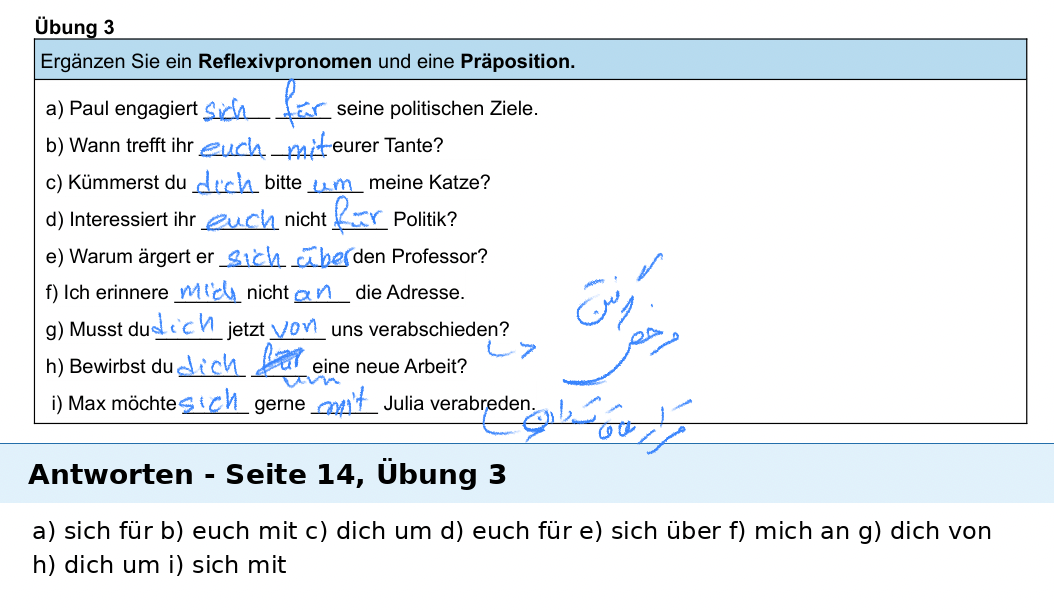
\includegraphics[width=0.9\textwidth]{s_14_u_3.png}
      \end{figure}
   \section{s_14_u_4}
      \begin{figure}[H]
         \centering
         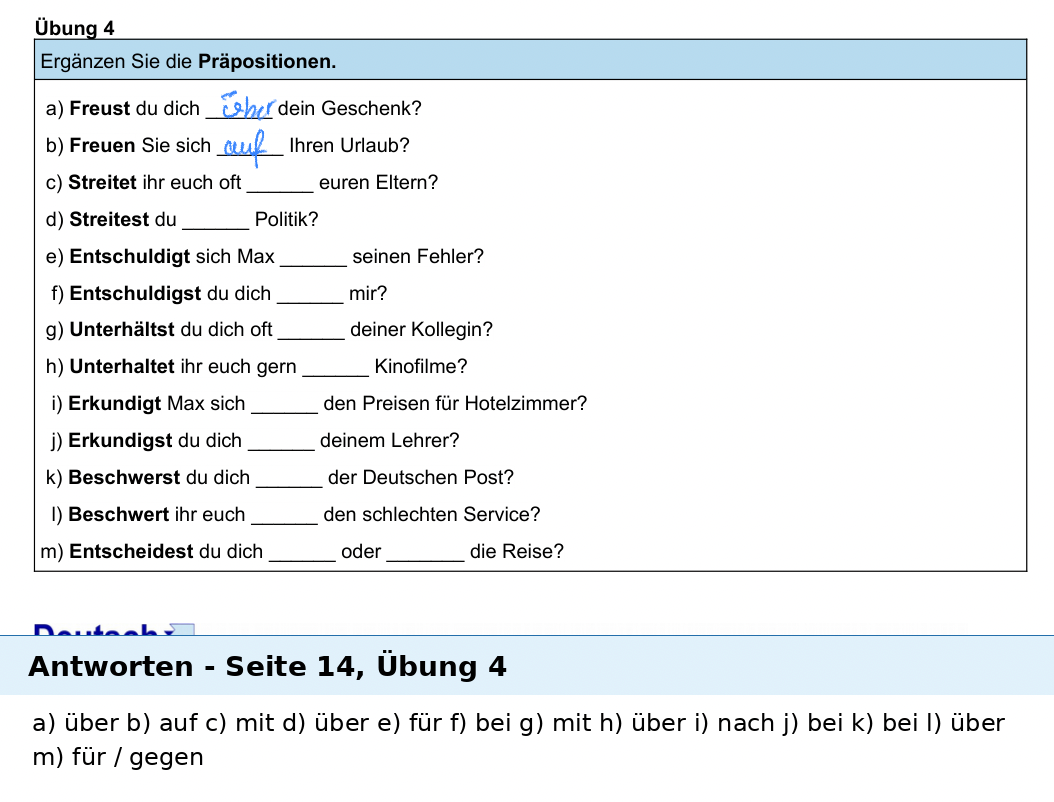
\includegraphics[width=0.9\textwidth]{s_14_u_4.png}
      \end{figure}
      \bibliographystyle{plainnat}
      \bibliography{/home/donkarlo/Dropbox/repo/nd_shared_research/bibliography/bibliography.bib}
\end{document}